\documentclass{article}

\usepackage[french]{babel}
\usepackage[utf8]{inputenc}
\usepackage[a4paper, margin=1in]{geometry}
\usepackage{graphicx}
\usepackage{hyperref}
\usepackage{amsmath}
\usepackage{siunitx}

\author{Marie Grange}
\date{\today}
\title{Propositions protocoles}

\begin{document}
	\maketitle %pour faire un comentaire
	\tableofcontents
	\pagebreak
	\section{Matériel générale}
	Personnel
	\begin{itemize}
		\item bottes
		\item chapeaux
		\item appareils photo (au moins 2)
	\end{itemize}
	A fournir
	\begin{itemize}
		\item crème solaire
		\item 2 parasols
		\item trousse de secourt
		\item (imprimante) + papier + ciseaux + scotche (étiquettes, fiches de terrain...)
		\item loupes
		\item 4 planches + pinces + pochettes plastiques
		\item 120 piquets 50cm (pour marquer l'extrémité des transects)
		\item 44 tuteurs (pour délimiter les transects)
		\item 1 ou 2 masses
		\item 1 ou 2 balances de terrain
	\end{itemize}

	\section{Organisation générale}
	
	Les relevés auront lieu dans la réserve du bout du lac d'Annecy et la réserve du marais de Giez, au sud du lac d'Annecy. 5 prairies ont été identifiées comme pertinentes pour l'étude. Elles ont été choisies de façon à présenter une flore comparable entre elles et à ce que chacune contienne des zones de forte, moyenne et faible présence et absence de S.canadensis. (\autoref{fig:loc-placettes})
	\begin{figure}[h]
		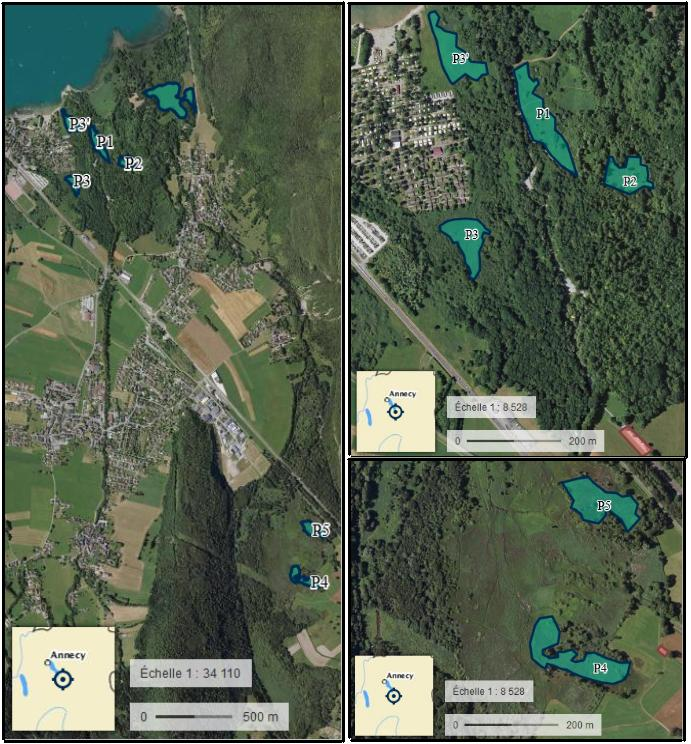
\includegraphics[width=\linewidth]{loc-placettes.jpg}
		\caption{Localisation des prairies (https://www.geoportail.gouv.fr/)}
		\label{fig:loc-placettes}
	\end{figure}
	\paragraph{} Au sein de chaque prairie, quatre placettes - homogènes du point de vue de la végétation - de 2500m$^2$ sont délimitées de façon à représenter un gradient de densité de S.canadensis (~0, ~100, ~200 et ~300 tiges/m$^2$, la densité dans des patchs bien établis pouvant atteindre 309 tiges/m$^2$ \cite{weber_biological_2000}). (\autoref{fig:disp-placettes})\\
	
	\begin{figure}[h]
		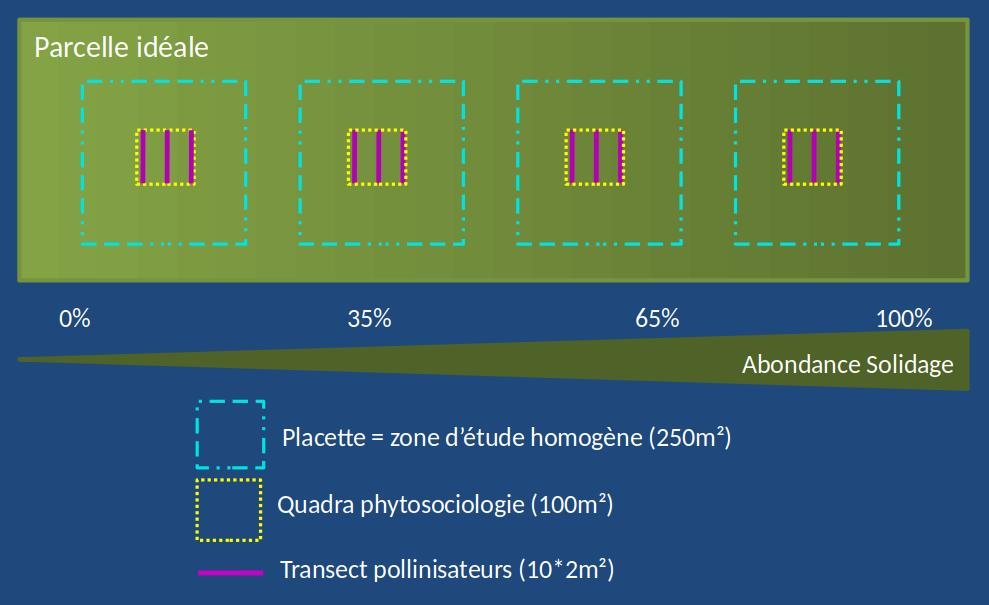
\includegraphics[width=\linewidth]{disp-placettes.jpg}
		\caption{Disposition des placettes dans chaque prairie}
		\label{fig:disp-placettes}
	\end{figure}

	\paragraph{} L'organisation des relevés au sein de ces placettes est présenté en \autoref{fig:disp-releves}

	\begin{figure}[h]
		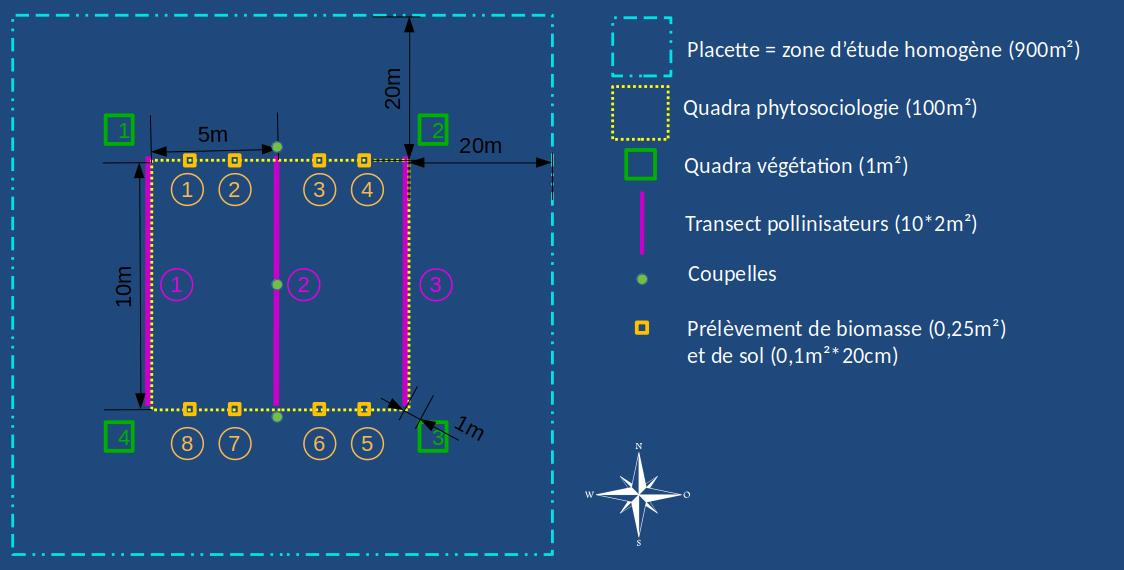
\includegraphics[width=\linewidth]{disp-releves.jpg}
		\caption{Disposition des relevés au sein de chaque placette}
		\label{fig:disp-releves}
	\end{figure}

	\pagebreak
	\section{Protocoles flore}
	
	\subsection{Relevé phytosocio}
	\subsubsection{Matériel}
	\begin{itemize}
		\item fiches des espèces connues sur la réserve
		\item fiche estimation des coefficients de Braun-Blanquet
		\item flores
		\item sacs congélation (échantillons) et étiquettes (date*placette*sp)
	\end{itemize}
	\subsubsection{Protocole}
	\begin{itemize}
		\item Relever la hauteur maximum de la végétation sur le quadra.
		\item Dresser la liste des espèces présentes (si travail sur tablette ou fiche non préremplie) en faisant parcourant les transects pollinisateurs. (\autoref{fig:disp-releves}). Les espèces non identifiées sont indiquées comme sp1, sp2...
		\item Pour chaque espèce, estimer l'indice d'abondance-recouvrement selon la méthode de Braun-Blanquet. (\underline{est-ce qu'on sépare 2 strates ~ prairie/mégaphorbiaie ?})
	\end{itemize}
	
	\subsection{Relevé quadras}
	\subsubsection{Matériel}
	\begin{itemize}
		\item 2 quadras (8m bois + 24 clous + 12m ficelle)
		\item fiches des espèces connues sur la réserve
		\item flores
		\item sacs congélation (échantillons) et étiquettes (date*placette*quadra*sp)
	\end{itemize}
	\subsubsection{Protocole}
	Dans les 4 angles de la station :
	\begin{itemize}
		\item Placer le quadra à 1m de la fin du transect (\autoref{fig:disp-releves})
		\item Dresser la liste des espèces présentes (si travail sur tablette ou fiche non préremplie) Les espèces non identifiées sont indiquées comme sp1, sp2...
		\item Pour chaque espèce, relever le nombre de sous-quadras (max=16) dans lesquels elle apparaît.
		\item Un ou plusieurs spécimens sont prélevés pour chaque espèce non identifiée et conservés dans un sac congélation avec étiquette (date*placette*quadra*sp).
	\end{itemize}
	
	\subsection{Sensibilité à la pollinisation}
	\subsubsection{Matériel}
	Pour la session de récolte :
	\begin{itemize}
		\item 500 capuchons
		\item agrafeuse
		\item 500 sachets de conservation
	\end{itemize}
	Pour l'analyse des taux de germination :
	\begin{itemize}
		\item ???
	\end{itemize}
	\subsubsection{Protocole}
	Pour chaque espèce cible (=espèces des expériences de compétition de Laure sauf le Dactyle) :
	\begin{itemize}
		\item avant floraison, "encapuchonner" 5 inflorescences d'individus différents dans chaque placette de densité 0 et 300 (soit 50 individus par espèce)
		\item en fin de floraison (mais avant déhiscence des fruits), 'encapuchonner" 5 inflorescences d'individus différents - si possible les mêmes qu'avant la floraison - dans chaque placette de densité 0 et 300 (soit 50 individus par espèce)
		\item lorsque les fruits sont tous arrivés à maturité, récolter les graines présentes dans les capuchons et les stocker dans des sachets de conservation individuels.
		\item compter, peser et stocker les graines (\underline{dans quelles conditions ?})
		\item au printemps (\underline{est-ce qu'on a des info sur comment lever la dormance pour ces espèces ?}), mettre les graines en terre (\underline{quelle bonne taille d'échantillon pour avoir une bonne estimation pour chaque individu ?}) et relever pendant (\underline{combien de temps ?}) le nombre de graines germées par individu.
	\end{itemize}
	\pagebreak
	
	\section{Protocoles insectes}
	
	\subsection{Relevé de la communauté prospectrice}
	Le protocole utilisé pour relever la communauté prospectrice d'insectes dans les stations est le protocole standardisé décrit par \cite{lebuhn_protocol_2016}. Ce protocole permet de maximiser l'efficacité du piégeage (entre 70\% et 95\% des espèces détectées), tout en limitant le coût et la durée des relevés (\cite{westphal_measuring_2008}). Ce protocole étant susceptible de biaiser les observations sur transects en augmentant l'attractivité des stations ou en concurrençant les fleurs, aucun autre relevé n'est effectué lorsqu'il est en place.
	\subsubsection{Matériel}
	\begin{itemize}
		\item 60 coupelles en plastic
		\item 60 tuteurs en bambou + masse
		\item 60 colliers de suspension perforés
		\item 60 visses + visseuse
		\item peinture fluo (jaune, bleu et blanc
		\item lessive
		\item 4 bidons d'eau (18 litres au total)
		\item 40 flacons de conservation
		\item 40 étiquettes (prairie*densité*couleur)
		\item alcool à $\SI{70}{\degree}$
	\end{itemize}
	\subsubsection{Protocole}
	Pendant la 3ème semaine de chaque session, lorsque la météo indique une absence de pluie et de vent pendant 2 jours :
	\begin{itemize}
		\item sur chaque transect 3 des placettes de densité 0 et 300, placer une coupelle de chaque couleur à 5m d'intervalle \underline{(cf LeBuhn 2016)}
		\item remplir les coupelles d'eau (300ml) et ajouter un peu de lessive
		\item revenir après 24h pour prélever tous les individus, les individus des coupelles blanches et bleu peuvent être mélangés (individus qui patrouillaient à la recherche de fleurs autres que le solidage)
	\end{itemize}
		En aval :
	\begin{itemize}
		\item épinglage des hyménoptères
		\item identification des apidae et syrphes au genre
		\item identification des lépidoptères à l'espèce si possible
		\item envoi des spécimens aux spécialistes pour identification à l'espèce
	\end{itemize}
	\pagebreak
	
	\subsection{Relevé des interactions de pollinisation}
	\subsubsection{Matériel}
	Pour toute la session :
	\begin{itemize}
		\item 24 piquets clôture amovible 
		\item 2 filets
		\item 2 glacières de terrain
		\item 1 glaciaire
		\item 2 besaces
		\item 300 flacons individuels (petits et très grands pour les lépidoptères)
		\item 24 sachets zip congélation (avec étiquettes des transects)
		\item 24 fiches terrain
		\item 2 fiches fleurs
		\item 2 fiches insectes protégés
	\end{itemize}
	Par passage :
	\begin{itemize}
		\item 10 flacons « de conservation » (20-30ml) préparés  avec copeaux de liège et acétate d’éthyl (donc 7200 flacons ~2,5 étages dans la salle des doctorants)
	\end{itemize}
	Pour la conservation et la préparation des insectes
	\begin{itemize}
		\item 4l alcool à $\SI{70}{\degree}$
		\item 1l acétate d'éthyl
		\item 2l copeaux de liège
		\item 12 000 épingles d'entomologie (2000 n.0, 2000 n.3 et 8000 n.1) 
		\item 2 000 minuties
		\item 2 000 plastazote
	\end{itemize}
	\subsubsection{Protocole}
	\begin{flushleft}
		En amont :
	\end{flushleft}
	\begin{itemize}
		\item Placement des transects
		\item Fiches identification fleurs
		\item Préparation des étiquettes (fleurs "plastifiées" et id passage)
	\end{itemize}
	Sur chaque transect :
	\begin{enumerate}
		\item Parcourir le transect une fois pour le fixer
		\item Relevé des espèces en fleur et de leur abondance (nombre d’inflorescences sur le transect)
		\item Pendant 15 minutes, relevé des interactions de pollinisation 
		\begin{itemize}
			\item marcher lentement le long du transect (~3 aller-retour par passage?) (obs1 devant, obs 2 derrière)
			\item quand insecte actif sur une fleure en vue (si plusieurs, toujours prélever le plus proche), obs1 annonce la fleure et attrape l'insecte au filet puis obs2 le transfère dans un flacon individuel avec l'étiquette de la fleure dans la glacière.
		\end{itemize}
		\item A la fin des 15 minutes, 
		\begin{itemize}
			\item \textit{(récupérer les piquets et les installer sur le transect suivant (obs1 et obs2))}
			\item prendre les lépidoptères en photo (face dorsale et ventrale des ailes), bien noter la référence des photos avec la plante, le transect et l’heure ! (obs1)
			\item noter le nombre d’abeilles domestiques récoltées sur chaque fleur puis les rassembler dans un grand flacon vide (obs2)
			\item rassembler dans flacons de conservation les hyménoptères (autres que apis mellifera), diptères et coléoptères par fleure avec étiquettes complètes (obs2)
		\end{itemize}
		\item A la pause suivante, relâcher les lépidoptères et abeilles domestiques (éviter de recapturer les mêmes individus sur le transect suivant) \textit{Pas d’impact sur la pop de mellifera, mais pour les lépidoptères ?}
	\end{enumerate}
	En aval :
	\begin{itemize}
		\item épinglage des hyménoptères
		\item identification des apidae et syrphes au genre
		\item identification des lépidoptères à l'espèce si possible
		\item envoi des spécimens aux spécialistes pour identification à l'espèce
	\end{itemize}
	\pagebreak

	\section{Protocoles services}
	\subsection{stockes de carbone}
	\underline Le fauchage pour évaluer la qualité fourragère est réalisé en juillet (date de fauche des prairies humides dans la région), les relevés pour le stock de C sont menés simultanément.
	\paragraph{}On s'intéresse à l'impact général sur le fourrage, mais aussi à l'impact sur la qualité fourragère de la communauté native (hyp : sélection des espèces très compétitives pour la lumière donc grandes donc à tige lignifiée)
	\subsubsection{Matériel}
	\begin{itemize}
		\item 2 (ou 4) quadras de 50*50cm
		\item 2 (ou 4) sécateurs ou tondeuses de terrain
		\item 2 (mini) râteaux 
		\item 2 bêches
		\item 2 tamis à 2mm
		\item 1 bassines
		\item 2 balances avec précision au gramme
		\item 80 sacs poubelle (20 grands et 60 petits)
		\item 80 sachets de conservation de 125ml
	\end{itemize}
	\subsubsection{Protocole}
	Sur chaque placette :
	\begin{itemize}
		\item mesurer la hauteur maximum de la végétation dans les 8 quadra et compter les tiges de S.canadensis
		\item récolter de la biomasse aérienne sur les 8 quadra dans les grands sacs poubelle (\underline{comment standardiser la hauteur de coupe ? : couper le plus ras possible / poser un quadra + baguette ?})
		\item récolter la litière restant au sol dans les 8 quadra dans les petits sacs poubelle
		\item prélever à la bêche une motte de 10*10*20cm \underline{(prévoir forme !)} au centre de 4 quadras dans les petits sacs poubelle
	\end{itemize}

	\paragraph{} Au gîte :
	\begin{itemize}
		\item peser la biomasse aérienne totale
		\item couper (\underline{mixer ?}), mélanger et  prélever un échantillon de 500g de biomasse aérienne 
		\item séparer de l'échantillon les parties jaunies, le re-peser et garder dans un sachet de conservation
		\item peser la litière et (séparément) les parties jaunies de la biomasse aérienne
		\item couper (\underline{mixer ?}) la litière et (séparément) les parties jaunies de la biomasse aérienne, mélanger et ré-échantillonner $\alpha * li$ de litière et $\alpha * baj$ de biomasse aérienne jaune. Mélanger les deux échantillons et les conserver dans un sachet.
		\item tamiser le sol pour séparer le sol, les éléments grossiers et les racines
		\item peser le sol, les éléments grossiers et les racines
		\item mélanger le sol et prélever un échantillon de 100g
		\item couper (\underline{mixer ?}), mélanger et  prélever un échantillon de 500g de biomasse souterraine
		\item faire sécher les échantillons (\underline{-> prévoir une table / une pièce dédiée !})
	\end{itemize}
 
	\paragraph{} Au labo :
	\begin{itemize}
		\item sécher les échantillon en étuve à \SI{55}{\degree} pendant 48h
		\item peser les échantillons secs
		\item broyer les échantillons
		\item passer les échantillons au CHN
	%	\item évaluation du processus de décomposition
	\end{itemize}
	\pagebreak
	
% 	\subsection{évaluation du processus de décomposition}
%	\paragraph{Matériel}
%	\begin{itemize}
%		\item 200 sachets en nylon (3g)
%		\item 20 microcosmes (3m de tuyau pvc 15*15cm + 40 coupelles + 1m$^2$ grillage fin) \underline{ou tupperwares ? }
%	\end{itemize}
%	\paragraph{Protocole} (\cite{fortunel_leaf_2009}\cite{kazakou_litter_2009})\\
%	\underline{Quelle date ?} Dans la littérature c'est toujours "au maximum de défoliation" mais comme beaucoup d'espèces et probablement une différence marquée entre les zones avec et sans solidage... J'aurai tendance à dire que le plus simple c'est de faire tout à la même date, à la fin de la saison de terrain... sauf que le Solidage sera encore en feuilles -> revenir en septembre/octobre pour une journée ? Sachant que la litière "d'été" aura potentiellement déjà disparue et sera donc sous-estimée.\\
%	\underline{Solution provisoire :} avec tous les relevés en juillet et analyser aussi la décomposition du "foin".\\
%	\underline{Service ou caractéristique du fonctionnement de l'écosystème ?} On peut considérer le processus de décomposition comme un service (c'est la différence entre avec et sans solidage qui nous intéresse) ou une caractéristique de l'écosystème qui est impliqué dans un cycle de rétroaction positive sur la population de S. canadensis favorisant sa colonisation en défavorisant les espèces qui ne supportent pas une litière épaisse / un humus riche. Les prairies échantillonnées étant fauchées avec export tous les ans, ce phénomène n'intervient pas dans ces prairies et ne peut donc être utilisé pour expliquer le succès de S.canadensis, mais doit être pris en compte dans une optique de modélisation ? \underline{donc on laisse tomber la décompo ?}
%	\begin{itemize}
%		\item laisser la litière sécher à température ambiante pendant 2 jours	
%		\item répartir chaque échantillon de litière dans 22(82) sachets de nylon de 3g
%		\item placer 2 des sachets en étuve à $\SI{55}{\degree}$C pendant 48h et peser pour estimer le poids sec des échantillons posés dans les microcosmes.
%		\item placer les autres sacs dans des béchers de 100(50?)ml d'eau
%		\item répartir chaque échantillon de sol entre 2(8) microcosmes et placer dans chacun 10 sachets (et l'eau correspondante) provenant d'un même échantillon de litière issus de la même prairie que le sol (cf schéma)
%		\item chaque semaine, ajouter x ml d'eau pour maintenir le sol à 80\% de sa capacité de champ. \underline{comment on sait où on en est ?}
%		\item aux semaines 1,2, 4, 6 et 8, prélever 2 sachets dans chaque microcosme
%		\item mettre les sachets à l'étuve 48h à $\SI{55}{\degree}$C.
%		\item peser les sachets
%	\end{itemize}
%	\paragraph{Analyse}
%	La masse sèche des sachets est supposée suivre une décroissance exponentielle de paramètre $\lambda$.(\cite{fortunel_leaf_2009}\cite{kazakou_litter_2009}) $$N(t)=N_{0}e^{-\lambda t}$$
%	Ce coefficient est comparé entre les différentes combinaisons de sol et de litière testées dans les microcosmes par ANOVA prenant en compte comme variables qualitatives la densité de S.canadensis associée au sol et celle associée à la litière.\\
%	L'expérience est construite pour pouvoir répondre à deux questions : 
%	\begin{itemize}
%		\item Quel est l'impact de S.canadensis sur la décomposabilité de la litière ?
%		\item Quel est l'impact de S.canadensis sur la capacité de dégradation de la matière organique des micro-organismes du sol ?
%	\end{itemize}
%	Un facteur d'interaction entre les 2 variables peut aussi être considéré dans la mesure où l'on peut faire l'hypothèse que si les litières sont très différenciés en fonction de l'abondance de S.canadensis, les micro-organismes du sol sont spécialisés dans la décomposition de la litière caractéristique de leur densité.
	\pagebreak	
	\bibliographystyle{apalike}
	\bibliography{mybib-proto.bib}
	
\end{document}